\documentclass{standalone}
\usepackage{tikz}
\usetikzlibrary{patterns, positioning}


\begin{document}
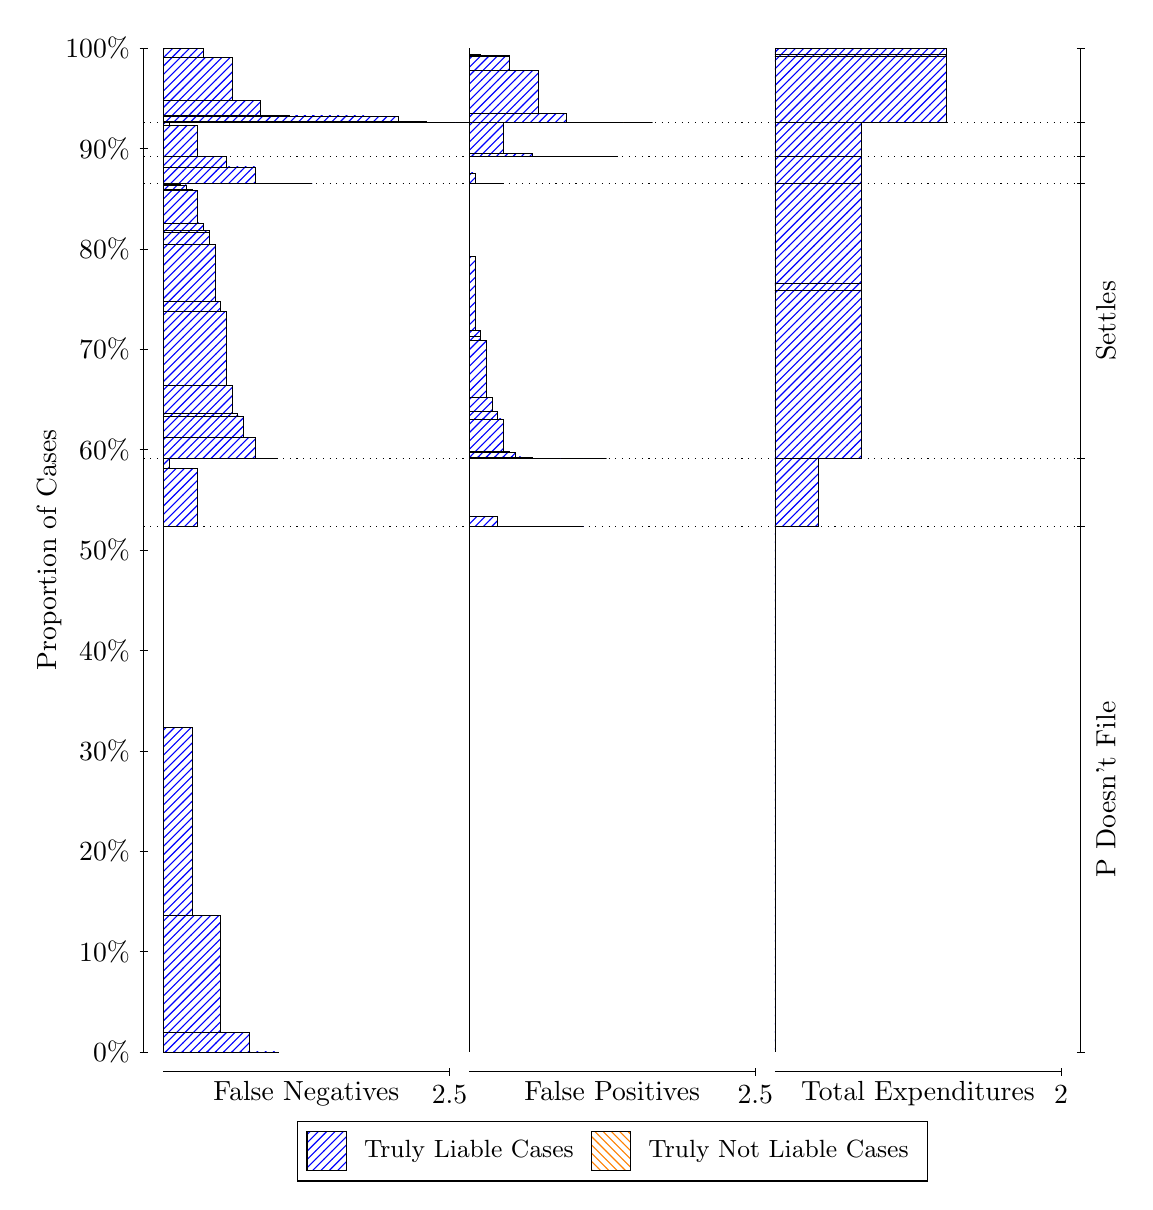
\begin{tikzpicture}
\draw[black, very thin] (1.5,1.75) -- (1.5,14.5);
\node[rotate=90, text=black, anchor=center] at (0.3, 8.125) {Proportion of Cases};
\draw[black, very thin] (1.45,1.75) -- (1.55,1.75);
\node[text=black, anchor=east] at (1.45, 1.75) {0\%};
\draw[black, very thin] (1.45,3.025) -- (1.55,3.025);
\node[text=black, anchor=east] at (1.45, 3.025) {10\%};
\draw[black, very thin] (1.45,4.3) -- (1.55,4.3);
\node[text=black, anchor=east] at (1.45, 4.3) {20\%};
\draw[black, very thin] (1.45,5.575) -- (1.55,5.575);
\node[text=black, anchor=east] at (1.45, 5.575) {30\%};
\draw[black, very thin] (1.45,6.85) -- (1.55,6.85);
\node[text=black, anchor=east] at (1.45, 6.85) {40\%};
\draw[black, very thin] (1.45,8.125) -- (1.55,8.125);
\node[text=black, anchor=east] at (1.45, 8.125) {50\%};
\draw[black, very thin] (1.45,9.4) -- (1.55,9.4);
\node[text=black, anchor=east] at (1.45, 9.4) {60\%};
\draw[black, very thin] (1.45,10.675) -- (1.55,10.675);
\node[text=black, anchor=east] at (1.45, 10.675) {70\%};
\draw[black, very thin] (1.45,11.95) -- (1.55,11.95);
\node[text=black, anchor=east] at (1.45, 11.95) {80\%};
\draw[black, very thin] (1.45,13.225) -- (1.55,13.225);
\node[text=black, anchor=east] at (1.45, 13.225) {90\%};
\draw[black, very thin] (1.45,14.5) -- (1.55,14.5);
\node[text=black, anchor=east] at (1.45, 14.5) {100\%};

\draw[black, very thin] (13.4,1.75) -- (13.4,14.5);
\draw[black, very thin] (13.35,1.75) -- (13.45,1.75);
\node[anchor=west] at (13.35, 1.75) {};
\draw[black, very thin] (13.35,8.4204) -- (13.45,8.4204);
\node[anchor=west] at (13.35, 8.4204) {};
\draw[black, very thin] (13.35,9.2919) -- (13.45,9.2919);
\node[anchor=west] at (13.35, 9.2919) {};
\draw[black, very thin] (13.35,12.778) -- (13.45,12.778);
\node[anchor=west] at (13.35, 12.778) {};
\draw[black, very thin] (13.35,13.128) -- (13.45,13.128);
\node[anchor=west] at (13.35, 13.128) {};
\draw[black, very thin] (13.35,13.552) -- (13.45,13.552);
\node[anchor=west] at (13.35, 13.552) {};
\draw[black, very thin] (13.35,14.5) -- (13.45,14.5);
\node[anchor=west] at (13.35, 14.5) {};

\draw[black, very thin, pattern color=blue, pattern=north east lines] (1.75,1.75) rectangle (3.2033,1.7525);
\draw[black, very thin, pattern color=blue, pattern=north east lines] (1.75,1.7525) rectangle (2.84,2.0033);
\draw[black, very thin, pattern color=blue, pattern=north east lines] (1.75,2.0033) rectangle (2.4767,3.4798);
\draw[black, very thin, pattern color=blue, pattern=north east lines] (1.75,3.4798) rectangle (2.1133,5.872);
\draw[black, very thin, pattern color=orange, pattern=north west lines] (1.75,5.872) rectangle (1.75,5.872);
\draw[black, very thin, pattern color=blue, pattern=north east lines] (1.75,5.872) rectangle (1.75,8.4204);
\draw[black, very thin, pattern color=blue, pattern=north east lines] (1.75,8.4204) rectangle (2.186,9.1615);
\draw[black, very thin, pattern color=blue, pattern=north east lines] (1.75,9.1615) rectangle (1.8227,9.2914);
\draw[black, very thin, pattern color=orange, pattern=north west lines] (1.75,9.2914) rectangle (1.75,9.2914);
\draw[black, very thin, pattern color=blue, pattern=north east lines] (1.75,9.2914) rectangle (1.75,9.2919);
\draw[black, very thin, pattern color=blue, pattern=north east lines] (1.75,9.2919) rectangle (3.2033,9.2919);
\draw[black, very thin, pattern color=blue, pattern=north east lines] (1.75,9.2919) rectangle (3.058,9.2921);
\draw[black, very thin, pattern color=blue, pattern=north east lines] (1.75,9.2921) rectangle (2.9127,9.5542);
\draw[black, very thin, pattern color=blue, pattern=north east lines] (1.75,9.5542) rectangle (2.84,9.5587);
\draw[black, very thin, pattern color=blue, pattern=north east lines] (1.75,9.5587) rectangle (2.7673,9.8274);
\draw[black, very thin, pattern color=blue, pattern=north east lines] (1.75,9.8274) rectangle (2.6947,9.8598);
\draw[black, very thin, pattern color=blue, pattern=north east lines] (1.75,9.8598) rectangle (2.622,10.214);
\draw[black, very thin, pattern color=blue, pattern=north east lines] (1.75,10.214) rectangle (2.5493,11.153);
\draw[black, very thin, pattern color=blue, pattern=north east lines] (1.75,11.153) rectangle (2.4767,11.279);
\draw[black, very thin, pattern color=blue, pattern=north east lines] (1.75,11.279) rectangle (2.404,12.007);
\draw[black, very thin, pattern color=blue, pattern=north east lines] (1.75,12.007) rectangle (2.3313,12.156);
\draw[black, very thin, pattern color=blue, pattern=north east lines] (1.75,12.156) rectangle (2.3313,12.18);
\draw[black, very thin, pattern color=blue, pattern=north east lines] (1.75,12.18) rectangle (2.2587,12.279);
\draw[black, very thin, pattern color=blue, pattern=north east lines] (1.75,12.279) rectangle (2.186,12.693);
\draw[black, very thin, pattern color=blue, pattern=north east lines] (1.75,12.693) rectangle (2.1133,12.7);
\draw[black, very thin, pattern color=blue, pattern=north east lines] (1.75,12.7) rectangle (2.0407,12.761);
\draw[black, very thin, pattern color=blue, pattern=north east lines] (1.75,12.761) rectangle (1.968,12.767);
\draw[black, very thin, pattern color=blue, pattern=north east lines] (1.75,12.767) rectangle (1.968,12.768);
\draw[black, very thin, pattern color=blue, pattern=north east lines] (1.75,12.768) rectangle (1.8953,12.769);
\draw[black, very thin, pattern color=blue, pattern=north east lines] (1.75,12.769) rectangle (1.8227,12.778);
\draw[black, very thin, pattern color=orange, pattern=north west lines] (1.75,12.778) rectangle (1.75,12.778);
\draw[black, very thin, pattern color=blue, pattern=north east lines] (1.75,12.778) rectangle (1.75,12.778);
\draw[black, very thin, pattern color=blue, pattern=north east lines] (1.75,12.778) rectangle (3.6393,12.778);
\draw[black, very thin, pattern color=blue, pattern=north east lines] (1.75,12.778) rectangle (3.276,12.785);
\draw[black, very thin, pattern color=blue, pattern=north east lines] (1.75,12.785) rectangle (2.9127,12.991);
\draw[black, very thin, pattern color=blue, pattern=north east lines] (1.75,12.991) rectangle (2.5493,13.126);
\draw[black, very thin, pattern color=blue, pattern=north east lines] (1.75,13.126) rectangle (2.186,13.128);
\draw[black, very thin, pattern color=orange, pattern=north west lines] (1.75,13.128) rectangle (1.75,13.128);
\draw[black, very thin, pattern color=blue, pattern=north east lines] (1.75,13.128) rectangle (2.186,13.518);
\draw[black, very thin, pattern color=blue, pattern=north east lines] (1.75,13.518) rectangle (1.8227,13.552);
\draw[black, very thin, pattern color=orange, pattern=north west lines] (1.75,13.552) rectangle (1.75,13.552);
\draw[black, very thin, pattern color=blue, pattern=north east lines] (1.75,13.552) rectangle (1.75,13.552);
\draw[black, very thin, pattern color=blue, pattern=north east lines] (1.75,13.552) rectangle (5.8193,13.552);
\draw[black, very thin, pattern color=blue, pattern=north east lines] (1.75,13.552) rectangle (5.456,13.552);
\draw[black, very thin, pattern color=blue, pattern=north east lines] (1.75,13.552) rectangle (5.0927,13.572);
\draw[black, very thin, pattern color=blue, pattern=north east lines] (1.75,13.572) rectangle (4.7293,13.636);
\draw[black, very thin, pattern color=blue, pattern=north east lines] (1.75,13.636) rectangle (4.366,13.637);
\draw[black, very thin, pattern color=blue, pattern=north east lines] (1.75,13.637) rectangle (4.0027,13.637);
\draw[black, very thin, pattern color=blue, pattern=north east lines] (1.75,13.637) rectangle (3.712,13.637);
\draw[black, very thin, pattern color=blue, pattern=north east lines] (1.75,13.637) rectangle (3.6393,13.637);
\draw[black, very thin, pattern color=blue, pattern=north east lines] (1.75,13.637) rectangle (3.3487,13.642);
\draw[black, very thin, pattern color=blue, pattern=north east lines] (1.75,13.642) rectangle (2.9853,13.832);
\draw[black, very thin, pattern color=blue, pattern=north east lines] (1.75,13.832) rectangle (2.622,14.38);
\draw[black, very thin, pattern color=blue, pattern=north east lines] (1.75,14.38) rectangle (2.2587,14.496);
\draw[black, very thin, pattern color=blue, pattern=north east lines] (1.75,14.496) rectangle (1.8953,14.5);
\draw[black, very thin, pattern color=orange, pattern=north west lines] (1.75,14.5) rectangle (1.75,14.5);
\draw[black, very thin, pattern color=blue, pattern=north east lines] (1.75,14.5) rectangle (1.75,14.5);
\draw[black, very thin, pattern color=orange, pattern=north west lines] (5.6333,1.75) rectangle (5.6333,1.75);
\draw[black, very thin, pattern color=blue, pattern=north east lines] (5.6333,1.75) rectangle (5.6333,8.4204);
\draw[black, very thin, pattern color=orange, pattern=north west lines] (5.6333,8.4204) rectangle (7.0867,8.4204);
\draw[black, very thin, pattern color=blue, pattern=north east lines] (5.6333,8.4204) rectangle (7.0867,8.4204);
\draw[black, very thin, pattern color=blue, pattern=north east lines] (5.6333,8.4204) rectangle (6.7233,8.4204);
\draw[black, very thin, pattern color=blue, pattern=north east lines] (5.6333,8.4204) rectangle (6.36,8.4209);
\draw[black, very thin, pattern color=blue, pattern=north east lines] (5.6333,8.4209) rectangle (5.9967,8.5508);
\draw[black, very thin, pattern color=blue, pattern=north east lines] (5.6333,8.5508) rectangle (5.6333,9.2919);
\draw[black, very thin, pattern color=orange, pattern=north west lines] (5.6333,9.2919) rectangle (7.3773,9.2919);
\draw[black, very thin, pattern color=blue, pattern=north east lines] (5.6333,9.2919) rectangle (7.3773,9.2919);
\draw[black, very thin, pattern color=orange, pattern=north west lines] (5.6333,9.2919) rectangle (7.232,9.2919);
\draw[black, very thin, pattern color=blue, pattern=north east lines] (5.6333,9.2919) rectangle (7.232,9.2919);
\draw[black, very thin, pattern color=orange, pattern=north west lines] (5.6333,9.2919) rectangle (7.0867,9.2919);
\draw[black, very thin, pattern color=blue, pattern=north east lines] (5.6333,9.2919) rectangle (7.0867,9.2919);
\draw[black, very thin, pattern color=blue, pattern=north east lines] (5.6333,9.2919) rectangle (7.014,9.2919);
\draw[black, very thin, pattern color=orange, pattern=north west lines] (5.6333,9.2919) rectangle (6.9413,9.2919);
\draw[black, very thin, pattern color=blue, pattern=north east lines] (5.6333,9.2919) rectangle (6.9413,9.2919);
\draw[black, very thin, pattern color=blue, pattern=north east lines] (5.6333,9.2919) rectangle (6.8687,9.2919);
\draw[black, very thin, pattern color=orange, pattern=north west lines] (5.6333,9.2919) rectangle (6.796,9.2919);
\draw[black, very thin, pattern color=blue, pattern=north east lines] (5.6333,9.2919) rectangle (6.796,9.2919);
\draw[black, very thin, pattern color=blue, pattern=north east lines] (5.6333,9.2919) rectangle (6.7233,9.2919);
\draw[black, very thin, pattern color=orange, pattern=north west lines] (5.6333,9.2919) rectangle (6.6507,9.2919);
\draw[black, very thin, pattern color=blue, pattern=north east lines] (5.6333,9.2919) rectangle (6.6507,9.2919);
\draw[black, very thin, pattern color=blue, pattern=north east lines] (5.6333,9.2919) rectangle (6.578,9.292);
\draw[black, very thin, pattern color=blue, pattern=north east lines] (5.6333,9.292) rectangle (6.5053,9.292);
\draw[black, very thin, pattern color=orange, pattern=north west lines] (5.6333,9.292) rectangle (6.5053,9.292);
\draw[black, very thin, pattern color=blue, pattern=north east lines] (5.6333,9.292) rectangle (6.5053,9.292);
\draw[black, very thin, pattern color=blue, pattern=north east lines] (5.6333,9.292) rectangle (6.4327,9.3009);
\draw[black, very thin, pattern color=blue, pattern=north east lines] (5.6333,9.3009) rectangle (6.36,9.3011);
\draw[black, very thin, pattern color=blue, pattern=north east lines] (5.6333,9.3011) rectangle (6.2873,9.3087);
\draw[black, very thin, pattern color=blue, pattern=north east lines] (5.6333,9.3087) rectangle (6.2147,9.37);
\draw[black, very thin, pattern color=blue, pattern=north east lines] (5.6333,9.37) rectangle (6.142,9.372);
\draw[black, very thin, pattern color=blue, pattern=north east lines] (5.6333,9.372) rectangle (6.142,9.376);
\draw[black, very thin, pattern color=blue, pattern=north east lines] (5.6333,9.376) rectangle (6.0693,9.7905);
\draw[black, very thin, pattern color=blue, pattern=north east lines] (5.6333,9.7905) rectangle (5.9967,9.8898);
\draw[black, very thin, pattern color=blue, pattern=north east lines] (5.6333,9.8898) rectangle (5.924,10.063);
\draw[black, very thin, pattern color=blue, pattern=north east lines] (5.6333,10.063) rectangle (5.8513,10.79);
\draw[black, very thin, pattern color=blue, pattern=north east lines] (5.6333,10.79) rectangle (5.7787,10.845);
\draw[black, very thin, pattern color=blue, pattern=north east lines] (5.6333,10.845) rectangle (5.7787,10.917);
\draw[black, very thin, pattern color=blue, pattern=north east lines] (5.6333,10.917) rectangle (5.706,11.855);
\draw[black, very thin, pattern color=blue, pattern=north east lines] (5.6333,11.855) rectangle (5.6333,12.778);
\draw[black, very thin, pattern color=orange, pattern=north west lines] (5.6333,12.778) rectangle (6.0693,12.778);
\draw[black, very thin, pattern color=blue, pattern=north east lines] (5.6333,12.778) rectangle (6.0693,12.779);
\draw[black, very thin, pattern color=blue, pattern=north east lines] (5.6333,12.779) rectangle (5.706,12.914);
\draw[black, very thin, pattern color=blue, pattern=north east lines] (5.6333,12.914) rectangle (5.6333,13.128);
\draw[black, very thin, pattern color=orange, pattern=north west lines] (5.6333,13.128) rectangle (7.5227,13.128);
\draw[black, very thin, pattern color=blue, pattern=north east lines] (5.6333,13.128) rectangle (7.5227,13.128);
\draw[black, very thin, pattern color=blue, pattern=north east lines] (5.6333,13.128) rectangle (7.1593,13.128);
\draw[black, very thin, pattern color=blue, pattern=north east lines] (5.6333,13.128) rectangle (6.796,13.128);
\draw[black, very thin, pattern color=blue, pattern=north east lines] (5.6333,13.128) rectangle (6.4327,13.162);
\draw[black, very thin, pattern color=blue, pattern=north east lines] (5.6333,13.162) rectangle (6.0693,13.552);
\draw[black, very thin, pattern color=orange, pattern=north west lines] (5.6333,13.552) rectangle (7.9587,13.552);
\draw[black, very thin, pattern color=blue, pattern=north east lines] (5.6333,13.552) rectangle (7.9587,13.552);
\draw[black, very thin, pattern color=orange, pattern=north west lines] (5.6333,13.552) rectangle (7.5953,13.552);
\draw[black, very thin, pattern color=blue, pattern=north east lines] (5.6333,13.552) rectangle (7.5953,13.552);
\draw[black, very thin, pattern color=orange, pattern=north west lines] (5.6333,13.552) rectangle (7.232,13.552);
\draw[black, very thin, pattern color=blue, pattern=north east lines] (5.6333,13.552) rectangle (7.232,13.556);
\draw[black, very thin, pattern color=blue, pattern=north east lines] (5.6333,13.556) rectangle (6.8687,13.672);
\draw[black, very thin, pattern color=orange, pattern=north west lines] (5.6333,13.672) rectangle (6.8687,13.672);
\draw[black, very thin, pattern color=blue, pattern=north east lines] (5.6333,13.672) rectangle (6.8687,13.672);
\draw[black, very thin, pattern color=blue, pattern=north east lines] (5.6333,13.672) rectangle (6.5053,14.218);
\draw[black, very thin, pattern color=blue, pattern=north east lines] (5.6333,14.218) rectangle (6.5053,14.219);
\draw[black, very thin, pattern color=blue, pattern=north east lines] (5.6333,14.219) rectangle (6.142,14.394);
\draw[black, very thin, pattern color=blue, pattern=north east lines] (5.6333,14.394) rectangle (6.142,14.41);
\draw[black, very thin, pattern color=blue, pattern=north east lines] (5.6333,14.41) rectangle (5.7787,14.414);
\draw[black, very thin, pattern color=blue, pattern=north east lines] (5.6333,14.414) rectangle (5.7787,14.415);
\draw[black, very thin, pattern color=orange, pattern=north west lines] (5.6333,14.415) rectangle (5.6333,14.415);
\draw[black, very thin, pattern color=blue, pattern=north east lines] (5.6333,14.415) rectangle (5.6333,14.5);
\draw[black, very thin, pattern color=orange, pattern=north west lines] (9.5167,1.75) rectangle (9.5167,1.75);
\draw[black, very thin, pattern color=blue, pattern=north east lines] (9.5167,1.75) rectangle (9.5167,8.4204);
\draw[black, very thin, pattern color=orange, pattern=north west lines] (9.5167,8.4204) rectangle (10.062,8.4204);
\draw[black, very thin, pattern color=blue, pattern=north east lines] (9.5167,8.4204) rectangle (10.062,9.2919);
\draw[black, very thin, pattern color=orange, pattern=north west lines] (9.5167,9.2919) rectangle (10.607,9.2919);
\draw[black, very thin, pattern color=blue, pattern=north east lines] (9.5167,9.2919) rectangle (10.607,11.426);
\draw[black, very thin, pattern color=orange, pattern=north west lines] (9.5167,11.426) rectangle (10.607,11.426);
\draw[black, very thin, pattern color=blue, pattern=north east lines] (9.5167,11.426) rectangle (10.607,11.507);
\draw[black, very thin, pattern color=orange, pattern=north west lines] (9.5167,11.507) rectangle (10.607,11.507);
\draw[black, very thin, pattern color=blue, pattern=north east lines] (9.5167,11.507) rectangle (10.607,12.778);
\draw[black, very thin, pattern color=orange, pattern=north west lines] (9.5167,12.778) rectangle (10.607,12.778);
\draw[black, very thin, pattern color=blue, pattern=north east lines] (9.5167,12.778) rectangle (10.607,13.128);
\draw[black, very thin, pattern color=orange, pattern=north west lines] (9.5167,13.128) rectangle (10.607,13.128);
\draw[black, very thin, pattern color=blue, pattern=north east lines] (9.5167,13.128) rectangle (10.607,13.552);
\draw[black, very thin, pattern color=orange, pattern=north west lines] (9.5167,13.552) rectangle (11.697,13.552);
\draw[black, very thin, pattern color=blue, pattern=north east lines] (9.5167,13.552) rectangle (11.697,14.397);
\draw[black, very thin, pattern color=orange, pattern=north west lines] (9.5167,14.397) rectangle (11.697,14.397);
\draw[black, very thin, pattern color=blue, pattern=north east lines] (9.5167,14.397) rectangle (11.697,14.415);
\draw[black, very thin, pattern color=orange, pattern=north west lines] (9.5167,14.415) rectangle (11.697,14.415);
\draw[black, very thin, pattern color=blue, pattern=north east lines] (9.5167,14.415) rectangle (11.697,14.5);
\draw[black, dotted] (1.5,8.4204) -- (13.4,8.4204);
\draw[black, dotted] (1.5,9.2919) -- (13.4,9.2919);
\draw[black, dotted] (1.5,12.778) -- (13.4,12.778);
\draw[black, dotted] (1.5,13.128) -- (13.4,13.128);
\draw[black, dotted] (1.5,13.552) -- (13.4,13.552);
\draw[black, very thin] (1.75,1.5) -- (5.3833,1.5);
\node[text=black, anchor=north] at (3.5667, 1.5) {False Negatives};
\draw[black, very thin] (5.3833,1.45) -- (5.3833,1.55);
\node[text=black, anchor=north] at (5.3833, 1.45) {2.5};

\draw[black, very thin] (5.6333,1.5) -- (9.2667,1.5);
\node[text=black, anchor=north] at (7.45, 1.5) {False Positives};
\draw[black, very thin] (9.2667,1.45) -- (9.2667,1.55);
\node[text=black, anchor=north] at (9.2667, 1.45) {2.5};

\draw[black, very thin] (9.5167,1.5) -- (13.15,1.5);
\node[text=black, anchor=north] at (11.333, 1.5) {Total Expenditures};
\draw[black, very thin] (13.15,1.45) -- (13.15,1.55);
\node[text=black, anchor=north] at (13.15, 1.45) {2};

\node[text=black, centered, rotate=90] at (13.72, 5.0852) {P Doesn't File};

\node[text=black, centered, rotate=90] at (13.72, 11.035) {Settles};




\draw (7.449999999999999,1.5) node[draw=none] (baseCoordinate) {};
\begin{scope}[align=center]
        \matrix[scale=0.5, draw=black, below=0.5cm of baseCoordinate, nodes={draw}, column sep=0.1cm]{
            \node[rectangle, draw, minimum width=0.5cm, minimum height=0.5cm, pattern color=blue, pattern=north east lines] {}; &
            \node[draw=none, font=\small, text=black] (B) {Truly Liable Cases}; &
            \node[rectangle, draw, minimum width=0.5cm, minimum height=0.5cm, pattern color=orange, pattern=north west lines] {}; &
            \node[draw=none, font=\small, text=black] (B) {Truly Not Liable Cases}; \\
            };
\end{scope}

\end{tikzpicture}
\end{document}